\begin{center}
    {\large\bfseries Непрерывная олимпиада. Решения}
\end{center}

\footnotesize

\begin{enumerate}
\item \textit{Найдите наибольшее чётное число,
которое делится на 75 и не содержит в
своей записи одинаковых цифр.}

В записи числа не больше десяти различных цифр. Любое десятизначное число
больше любого числа с меньшим количеством цифр, поэтому используем все цифры
от 0 до 9.

Чётное число, кратное 25, должно оканчиваться на 00 или 50. Окончание 00
не подходит, так как цифры не должны повторяться. Значит, число оканчивается
на 50. Сумма всех его цифр равна $45$, поэтому оно делится на 3. Чтобы число
было наибольшим, остальные цифры записываем в порядке убывания.

\textit{Ответ:} 9876432150.

\item \textit{Разрежьте фигуру на трёхклеточные уголки так, чтобы в каждом
уголке было по кружочку.}

Один из вариантов разрезания:

\begin{center}
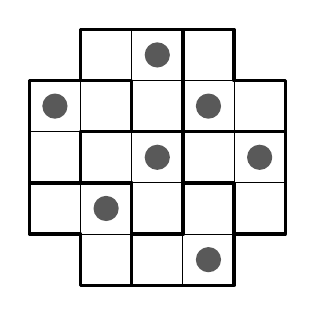
\begin{tikzpicture}[x=0.65cm,y=0.65cm,line join=round]
    \foreach \x in {1,2,3} {
        \draw[line width=0.35pt] (\x,0) rectangle ++(1,-1);
        \draw[line width=0.35pt] (\x,-4) rectangle ++(1,-1);
    }
    \foreach \y in {-1,-2,-3} {
        \foreach \x in {0,1,2,3,4} {
            \draw[line width=0.35pt] (\x,\y) rectangle ++(1,-1);
        }
    }

    \draw[line width=1.2pt] (1,0)--(3,0)--(3,-2)--(2,-2)--(2,-1)--(1,-1)--cycle;
    \draw[line width=1.2pt] (3,0)--(4,0)--(4,-1)--(5,-1)--(5,-2)--(3,-2)--cycle;
    \draw[line width=1.2pt] (0,-1)--(2,-1)--(2,-2)--(1,-2)--(1,-3)--(0,-3)--cycle;
    \draw[line width=1.2pt] (1,-2)--(3,-2)--(3,-4)--(2,-4)--(2,-3)--(1,-3)--cycle;
    \draw[line width=1.2pt] (3,-2)--(5,-2)--(5,-4)--(4,-4)--(4,-3)--(3,-3)--cycle;
    \draw[line width=1.2pt] (0,-3)--(2,-3)--(2,-5)--(1,-5)--(1,-4)--(0,-4)--cycle;
    \draw[line width=1.2pt] (3,-3)--(4,-3)--(4,-5)--(2,-5)--(2,-4)--(3,-4)--cycle;

    \foreach \p in {(2.5,-0.5),(0.5,-1.5),(3.5,-1.5),
                     (2.5,-2.5),(4.5,-2.5),(1.5,-3.5),(3.5,-4.5)} {
        \fill[black!65] \p circle[radius=0.16cm];
    }
\end{tikzpicture}
\end{center}

\item \textit{Во фруктовой лавке есть пять дынь
различного веса, каждая весит целое
число килограммов. Две самые тяжёлые
дыни весят в два раза больше остальных
трёх, а три самые тяжёлые дыни весят в
восемь раз больше остальных двух.
Найдите наименьшее возможное
значение суммарного веса всех дынь.}

Пусть две самые лёгкие дыни вместе весят $s$ кг. Их веса --- различные
натуральные числа, поэтому $s\geqslant1+2=3$. Три самые тяжёлые дыни весят
$8s$ кг, а все пять --- $9s\geqslant27$ кг.

Оценка достигается для весов $1$, $2$, $6$, $7$ и $11$ кг:
\[
7+11=2(1+2+6), \qquad 6+7+11=8(1+2).
\]

\textit{Ответ: } 27 кг.
\end{enumerate}
